\chapter{Partnerdatenbank}
Im Folgenden werden der Grundaufbau und Zweck der Partnerdatenbank sowie die Funktionsweise des Backends und des Frontends beschrieben.

\section{Grundaufbau und Zweck der Partnerdatenbank}
Die 3 Banken IT GmbH verwaltet ihre Partner in verschiedenen Systemen. Dazu gehören die Art28\_Verträge\_Fernwartungszugänge\_VPE-Liste, in der die Angebotsanfragen und die Ausschreibungen dokumentiert sind und die FiPe-Liste, in der Kontaktpartner mit Kürzel, Name und laufender Nummer erfasst sind. Beide Listen sollen durch die Partnerdatenbank abgelöst werden.

Die Partnerdatenbank ist ein Prototyp für die 3 Banken IT GmbH, um zukünftig ihre Partner sowie ihre Anwendungsfälle besser zu managen. In diesem Prototyp werden die Anwendungsfälle, die  in der Abbildung \ref{fig:UseCaseDiagramm} zu sehen sind, \textit{Unternehmen anlegen}, \textit{Kontaktperson anlegen}, \textit{Unternehmen anzeigen} und \textit{Kontaktperson anzeigen}, implementiert.
Grundsätzlich kann jeder Mitarbeiter diese vier Geschäftsfälle erledigen, sofern dieser eingeloggt ist.

Dieser Login wird rollenbasiert implementiert. Das bedeutet, dass in Zukunft Geschäftsfälle auch nur von bestimmten Usern mit bestimmten Rollen durchgeführt werden können.
Alle REST-Aufrufe, außer dem Login, können lediglich als eingeloggter User aufgerufen werden.

Die Partnerdatenbank dient auch als Anreiz und Motivation für die 3 Banken IT GmbH, zukünftig Anwendungen mit Microservice-Architekturen zu entwickeln. Diese Form der Architektur bietet, wie bereits beschrieben, sehr viele Vorteile bei der Abwicklung von Geschäftsprozessen.

\begin{figure}[h]
	\begin{center}
		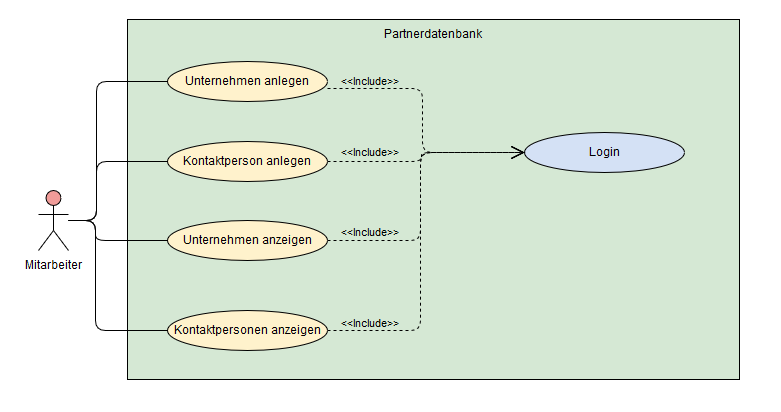
\includegraphics[scale=0.70]{Partnerdatenbank_UseCases.png}
		\caption[Anwendungsfalldiagramm der Partnerdatenbank]{Anwendungsfalldiagramm der Partnerdatenbank}
		\label{fig:UseCaseDiagramm}
	\end{center}
\end{figure}


\subsection{Lifecycle der Daten}
Weitere Geschäftsprozesse, welche die Daten der 3 Banken IT GmbH durchlaufen und in die Partnerdatenbank integriert werden, sind:
\begin{enumerate}
	\item Erstkontakt,
	\item Angebotsanfrage/Ausschreibung,
	\item Angebotslegung,
	\item Verpflichtungserklärung,
	\item Auftrag,
	\item Lieferung,
	\item Rechnung,
	\item Installation,
	\item Inbetriebnahme,
	\item Kündigung,
	\item Deaktivierung,
	\item Deinstallation.
\end{enumerate}

Diese werden jedoch nicht vom Ersteller dieser Anwendung integriert, sondern von der 3 Banken IT GmbH selbst. Diese Arbeit dient lediglich als Vorlage und Schablone für die 3 Banken IT GmbH zur Integration weiterer Services bzw. Geschäftsfälle.

\section{Beschreibung der Datenbank}
Die Datenbanken für die 3 Banken IT GmbH bestehen aus Microsoft SQL Server-Datenbanken. Ein  Microsoft SQL Server ist ein relationales Datenbankmanagementsystem (DBMS), das von Microsoft entwickelt wurde. Dieses DBMS wurde von der 3 Banken IT GmbH vorgegeben. Der Verfasser dieser Arbeit beschreibt deshalb die Charakteristiken und Vor- und Nachteile dieses DBMS nicht genauer.

\subsection{Lokale Entwicklung}
Die Datenbank wird lokal über das in Listing \ref{lst:Dockerfile.local} dargestellte Dockerfile definiert.
\begin{lstlisting}[language=docker, caption=Dockerfile für die lokale Entwicklung, label={lst:Dockerfile.local}]
	FROM mcr.microsoft.com/mssql/server:2017-latest
	EXPOSE 1433
	COPY ./create-db.sql .
	USER root
	ENV MSSQL_DEVELOPER=sa
	ENV MSSQL_SA_PASSWORD=Ruhsi@1234
	ENV ACCEPT_EULA=Y
	RUN chgrp -R 0 /var/opt && \
		chmod -R g=u /var/opt && \
		chown -R 10001:0 /var/opt && \
		( /opt/mssql/bin/sqlservr --accept-eula & ) | \
			grep -q "Service Broker manager has started" && \
		/opt/mssql-tools/bin/sqlcmd -S localhost -U \
			sa -P Ruhsi@1234 -d master -i create-db.sql
\end{lstlisting}

Im Folgenden werden die Befehle des Dockerfiles beschrieben:
\begin{enumerate}
	\item Der \textbf{FROM}-Befehl definiert das Basis Image, das bereits einen vollständigen MS SQL Server beinhaltet. Dieses Image ist in der Registry von Microsoft zu finden und kann einfach verwendet werden.
	\item Der \textbf{EXPOSE}-Befehl gibt den Port 1433 des Containers nach außen frei, sodass auch externe Clients auf dieses Service Zugriff haben.
	\item Der \textbf{COPY}-Befehl kopiert die \textit{create-db.sql}-Datei in den Container. Diese Datei muss unter dem angegebenen Pfad verfügbar sein und enthält in diesem Fall lediglich zwei Zeilen (Listing \ref{lst:create-sql}).
\begin{lstlisting}[language=sql, caption=create-db.sql, label=lst:create-sql]
	CREATE DATABASE PartnerDB;
	CREATE DATABASE DocsisDB;
\end{lstlisting}
	Zur Speicherung der Partner sowie Unternehmen ist die \textit{PartnerDB} vorgesehen. Für die Speicherung der Links der Partner zu den entsprechenden Dokumenten ist die \textit{DocsisDB} vorgesehen. Die Dokumente zu den Partnern kommen aus dem Docsis-System der 3 Banken IT GmbH. Da der Verfasser auf dieses System keinen Zugriff hat, wurde beschlossen, dass die Daten in einer eigenständigen Datenbank gemockt werden.
	\item Der \textbf{USER}-Befehl setzt den User, mit dem die darauffolgenden Befehle ausgeführt werden. In diesem Fall wird der root-User verwendet, da laut Dokumentation dieses Basis Image nur mit Root-Rechten ausgeführt werden kann.
	\item Der \textbf{ENV}-Befehl setzt Environment-Variablen. Die beiden Environment-Variablen \textit{MSSQL\_DEVELOPER} und \textit{MSSQL\_SA\_PASSWORD} setzen die Login-Parameter, mit denen auf den SQL-Service zugegriffen werden kann. Mit der Environment-Variable \textit{ACCEPT\_EULA} wird das \glqq \href{https://documentation.commvault.com/commvault/v11/article?p=50060.htm}{End-User License Agreement}\grqq akzeptiert.
	\item Im \textbf{RUN}-Befehl werden gleich mehrere Schritte ausgeführt. Die Befehle in Zeile 8, 9 und 10 setzen den Besitzer der Dateien und Unterordner des angegebenen Pfades und gewähren ihm Zugriff auf alle Dateien darin. Dadurch können die Befehle in Zeile 11 und 12 mit dem root-User ausgeführt werden.
	\item Der Befehl in Zeile 11 startet den MS SQL Server und akzeptiert das EULA. Danach wird mit dem grep-Befehl solange gewartet, bis der SQL Server hochgefahren ist und in den Logs die Ausgabe \glqq Service Broker manager has started\grqq{} zu sehen ist.
	\item In Zeile 12 verbindet sich der User mithilfe des sqlcmd-Tools und den angegebenen Parametern zum MS SQL Server und führt das oben angeführte \textit{create-db.sql}-Skript aus.
\end{enumerate}

Dieses Dockerfile kann mit folgendem Befehl gebaut werden:
\begin{lstlisting}[language=bash]
$ docker build -t docsisdb .
\end{lstlisting}
Der Parameter \textit{-t docsisdb} vergibt einen Namen für das Image. Der Punkt am Ende des Befehls ist der Pfad zum Dockerfile, in diesem Fall wird der Befehl im selben Verzeichnis wie das Dockerfile ausgeführt.

Mit dem Befehl:
\begin{lstlisting}[language=bash]
$ docker run -d -p 1434:1433 --name docsisdb docsisdb
\end{lstlisting}
wird ein Docker Container aus dem Docker Image gestartet. Die Option \textit{-d} startet den Container im Hintergrund (detached). Die Option \textit{-p 1434:1433} leitet alle Aufrufe des Ports 1434 auf den container-internen Port 1433 weiter. Auf diesem Port ist der MS SQL Server erreichbar. Mit der Option \textit{-{}-name docsisdb} wird dem Docker Container der Name \glqq docsisdb\grqq{} zugewiesen. Dadurch startet der Docker Container und der MS SQL Server ist unter dem Port 1434 des Hosts verfügbar.

Zum vereinfachten Ausführen mehrerer Docker Container ist es bei Docker auch möglich ein \textit{docker-compose.yml} zu definieren, in dem mehrere Services definiert und ausgeführt werden.
In der Datei in Listing \ref{lst:docker-compose.yml} wird das docker-compose.yml zum Ausführen der beiden Dockerfiles der docsis-database und der partner-database beschrieben:
\begin{lstlisting}[language=docker-compose-2, caption={docker-compose.yml}, label=lst:docker-compose.yml]
	version: '3'
	services:
		partner-database:
			build: ./partner-database
			container_name: "partner-database"
			ports:
				- 1433:1433
	
		docsis-database:
			build: ./docsis-database
			container_name: "docsis-database"
			ports:
				- 1434:1433
\end{lstlisting}
Im \textbf{build} wird der Pfad zu den jeweiligen Dockerfiles gesetzt. Mit \textbf{container\_name} kann der Name des Containers gesetzt werden und im \textbf{ports}-Abschnitt werden die Ports freigegeben.

Mit dem Befehl:
\begin{lstlisting}[language=bash]
	$ docker-compose up
\end{lstlisting}
werden nun beide Docker Container gestartet und sind unter den jeweiligen Ports aufrufbar.

Die beiden Docker Container können mit folgendem Befehl wieder beendet werden:
\begin{lstlisting}[language=bash]
	$ docker-compose down
\end{lstlisting}

\subsection{Deployment in OpenShift}
Das Dockerfile und die create-db.sql-Datei sehen beim Deployment der Datenbank in OpenShift gleich aus. Sie verändern sich nicht. Dadurch ist sichergestellt, dass sich die Umgebungen lokal und in OpenShift gleich verhalten. Das Deployment gestaltet sich jedoch etwas aufwändiger als lediglich ein \glqq docker run\grqq-Befehl. Da es für MS SQL Server kein vordefiniertes Template in OpenShift gibt, muss das Docker Image in die OpenShift-interne Docker Registry gepusht werden.

Folgende Schritte müssen dafür unternommen werden:
\begin{enumerate}
	\item \textbf{Freigeben der Route}: Die OpenShift-interne Docker Registry muss nach außen freigegeben werden, um diese von der CLI aus aufzurufen. Dies kann in der Web Console von OpenShift von einem Administrator erledigt werden.
	\item \textbf{Holen der Route}: Mit dem Befehl:
\begin{lstlisting}[language=bash]
	$ oc get route
\end{lstlisting}
	kann die Route der Docker Registry geholt werden.
	\item \textbf{Einloggen in die Docker Registry}: Mit dem Befehl:
\begin{lstlisting}[language=bash]
	$ docker login -u <openshift_username> -p <openshift_password> 
		<registry_route>
\end{lstlisting}
	erfolgt der Login in die die OpenShift-interne Docker Registry.
	\item \textbf{Bauen des Docker Images lokal}: Mit folgendem Befehl wird das Docker Image mit dem Namen mssql versehen und gebaut:
\begin{lstlisting}[language=bash]
	$ docker build -t mssql .
\end{lstlisting}
	\item \textbf{Taggen des Images in der Registry}: Mit dem Befehl:
\begin{lstlisting}[language=bash]
	$ docker tag mssql <registry_route>/<namespace>/mssql
\end{lstlisting}
	wird ein Tag in der OpenShift-internen Registry erstellt. Dadurch wird eine Referenz des lokalen Docker Images zum OpenShift-internen Docker Image erstellt.
	\item \textbf{Pushen des Images in die Registry}: Durch den Befehl:
\begin{lstlisting}[language=bash]
	$ docker push <registry_route>/<namespace>/mssql
\end{lstlisting}
	wird das Docker Image in die OpenShift-interne Registry gepusht.
	Dadurch kann das Docker Image in OpenShift referenziert und ausgeführt werden.
	\item \textbf{Ausführen des Image}: Mit folgendem Befehl kann das Docker Image in OpenShift gebaut werden:
\begin{lstlisting}[language=bash]
	$ oc new-app mssql
\end{lstlisting}
	Dadurch wird der Docker Container in OpenShift ausgeführt und kann intern durch die Route \textit{mssql:1433} erreicht werden. Muss die App auch von extern erreicht werden können, muss die Route vorher freigegeben werden. Dies kann einfach über die Web Console erreicht werden.
\end{enumerate}

\section{Backend-Beschreibung}
In diesem Abschnitt wird der grundsätzliche Aufbau einer Backend-Applikation beschrieben.

\subsection{Paketstruktur}
In Abbildung \ref{fig:package_structure_partner_service} ist die Paketstruktur des \textit{partner-services} zu sehen.

Im Folgenden werden die wichtigsten Pakete näher beschrieben:
\begin{itemize}
	\item \textbf{src.main}
	\begin{itemize}
		\item \textbf{fabric8}:
		\begin{itemize}
			\item  Im \textit{fabric8}-Ordner befinden sich das \textbf{deployment.yml} und das \textbf{route.yml}, die für das Deployment in OpenShift notwendig sind. Diese werden in einem späteren Abschnitt näher beschrieben.
		\end{itemize}
		\item \textbf{java.at.fh.se.master.partner}
		\begin{itemize}
			\item \textbf{aspects}: In diesem Paket befindet sich die Klasse \textit{LoggingAspect.java}, die für das Logging jeder Methode im Paket \textbf{rest} zuständig ist.
			\item \textbf{configuration}: In diesem Paket befindet sich die Klasse \textit{SimpleCORSFilter.java}. Diese setzt die Origin-Header, damit das Frontend auf die Ressourcen zugreifen kann.
			\item \textbf{rest}: Im rest-Paket befinden sich die Interfaces und Implementierungen der REST-Api. Auch die Repositories für den Zugriff auf die Datenbank und eine \textit{RestTemplateProvider}-Klasse, die das RestTemplate für REST-Aufrufe zum Docsis-Service zu Verfügung stellt, sind in diesem Paket enthalten. 
			\item \textbf{security}: In diesem Paket sind die Sicherheitskonfigurationen für den Login und die weiteren authentifizierten Aufrufe enthalten. Zudem sind Modelklassen für den User und die Rolle enthalten.
			\item \textbf{service}: In diesem Paket ist ein Service für die Interaktion mit dem Docsis-Service enthalten. Damit können alle Links von einem Partner geholt, hinzugefügt und gelöscht werden.
		\end{itemize}
		\item \textbf{resources}
		\begin{itemize}
			\item In diesem Paket ist die Datei \textit{application.yml} enthalten, die zur Konfiguration der Applikation benötigt wird. Diese wird später näher erläutert.
		\end{itemize}
	\end{itemize}
	\item \textbf{src.test}
	\begin{itemize}
		\item \textbf{java.at.fh.se.master.partner}
		\begin{itemize}
			\item \textbf{rest.controller}:
			\begin{itemize}
				\item In diesem Paket befinden sich die Tests für die Controller-Klassen.
			\end{itemize}
		\end{itemize}
	\end{itemize}
\end{itemize} 

\begin{figure}[H]
	\begin{center}
		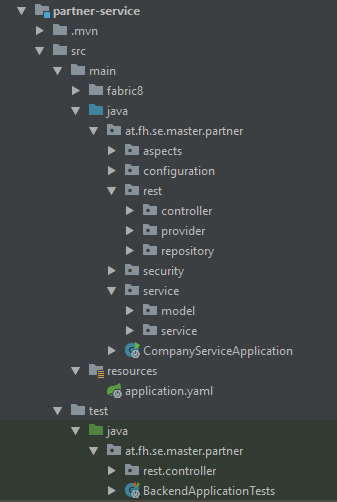
\includegraphics[scale=0.80]{package_structure_partner_service.png}
		\caption[Paketstruktur des Partnerservices]{Paketstruktur des Partnerservices}
		\label{fig:package_structure_partner_service}
	\end{center}
\end{figure}

\subsection{Logging}
Das Logging wird mithilfe von aspektorientierter Programmierung gelöst. Aspektorientierte Programmierung ist ein Paradigma, das darauf abzielt, die Modularität von Applikationen zu erhöhen. Dadurch wird zusätzliches Verhalten zum Code hinzugefügt, ohne den eigentlichen Code verändern zu müssen. Der neue Code und das zusätzliche Verhalten werden getrennt voneinander deklariert. 

In diesem Service wird aspektorientierte Programmierung zum Loggen der Ausführung von REST-Methoden genutzt. Dazu wird die Maven-Dependency in Listing \ref{lst:springbootstarteraop} benötigt.

\begin{lstlisting}[language=xml, caption=pom.xml, label=lst:springbootstarteraop]
	<dependency>
		<groupId>org.springframework.boot</groupId>
		<artifactId>spring-boot-starter-aop</artifactId>
	</dependency>
\end{lstlisting}

Die Deklaration des Aspekts sieht, wie in Listing \ref{lst:LoggingAspect} dargestellt, aus.

\begin{lstlisting}[language=java, caption={LoggingAspect.java}, label=lst:LoggingAspect]
	@Aspect
	@Component
	public class LoggingAspect {
		@Around("execution(public * at.fh.se.master.partner.rest..*(..))")
		public Object profileAllMethods(ProceedingJoinPoint proceedingJoinPoint);
	}
\end{lstlisting}

Die Klasse wird mit der Annotation \textit{@Aspect} als Aspekt gekennzeichnet. In der Klasse selbst wird ein Around-Advice deklariert. Dadurch werden alle public-Methoden mit jeglichem Rückgabeparameter im Verzeichnis \textit{at.fh.se.master.partner.rest} geloggt. Statt dem eigentlichen Aufruf der Methode wird der Aspekt aufgerufen. In diesem erfolgt das Logging. Danach muss die eigentliche Methode ausgeführt werden. Über den Parameter \textit{ProceedingJoinPoint proceedingJoinPoint} können Informationen über die Methodensignatur geholt werden. Über diesen Parameter kann auch die eigentliche Methode aufgerufen werden. Der Rückgabewert der eigentlichen Methode wird auch im Advice zurückgegeben.

\subsection{CORS-Filter}
Um einen Cross-Origin Resource Sharing (CORS)-Fehler beim Aufruf vom Frontend zu vermeiden, muss ein CORS-Filter implementiert werden. Dazu kann einfach das Interface \textit{Filter} implementiert werden. Danach muss die Methode \textit{doFilter} überschrieben werden. In dieser können die entsprechenden Header gesetzt werden.

Die Implementierung dazu zeigt Listing \ref{lst:SimpleCORSFilter}.
\begin{lstlisting}[language=java, caption={SimpleCORSFilter.java}, label=lst:SimpleCORSFilter]
	@Component
	public class SimpleCORSFilter implements Filter {
		@Override
		public void doFilter(ServletRequest req, ServletResponse resp,
		FilterChain chain) throws IOException, ServletException {
			HttpServletResponse response = (HttpServletResponse) resp;
			HttpServletRequest request = (HttpServletRequest) req;
			response.setHeader("Access-Control-Allow-Origin", request.getHeader("Origin"));
			...
		}
	}
\end{lstlisting}

Durch die beiden Parameter \textit{ServletRequest req} und \textit{ServletResponse resp} kann auf Informationen des Http-Requests und der Http-Response zugegriffen werden.
In diesem Prototyp wird der Header \textit{Access-Control-Allow-Origin} der Response mit dem Request-Header \textit{Origin} gesetzt. Dies erlaubt jeder Domain Zugriff auf diesen Server. Dies muss von der 3 Banken IT GmbH natürlich auf die entsprechende Domäne, in der das Frontend in der Produktivumgebung läuft, geändert werden.

\subsection{Controller}
Mit Controllern kann eine REST-Api bereitgestellt werden. Mit \textit{@RequestMapping} wird der grundsätzliche Pfad zu diesem Controller gesetzt. Die Annotation \textit{@CrossOrigin} ist ein Mechanismus, der von Spring Boot bereitgestellt wird und beim Handling von CORS unterstützt. Diese Annotation kann auch auf Klassenebene verwendet werden.
Durch die Annotation \textit{@PostMapping} wird die Methode als POST-Aufruf definiert. Diese ist in diesem Beispiel unter dem Pfad \glqq company\grqq{} verfügbar. Der Body des Requests muss in der Form von JSON vorliegen und diese Methode liefert auch Responsedaten in Form von JSON zurück. Die beiden Annotationen \textit{@ResponseBody} und \textit{@RequestBody} mappen den Rückgabewert bzw. den Inputparameter zu JSON. 
Der Inputparameter darf aufgrund der Annotation \textit{@NotNull} nicht null sein. Dieser muss auch durch die \textit{@Valid}-Annotation valide sein. In der Klasse Company können für einzelne Member Beschränkungen angegeben werden. Diese werden durch die Annotation @Valid validiert. Ein Beispiel für einen Controller zeigt Listing \ref{lst:CompanyControllerApi}.

\begin{lstlisting}[language=java, caption=CompanyControllerApi.java, label=lst:CompanyControllerApi]
	@RequestMapping("/")
	public interface CompanyControllerApi {
		...
	
		@CrossOrigin
		@PostMapping(value = "company",
			produces = MediaType.APPLICATION_JSON_VALUE,
			consumes = MediaType.APPLICATION_JSON_VALUE)
		@ResponseBody
		ResponseEntity<Company> addCompany(@RequestBody @NotNull 
			@Valid Company company);
		
		...
	}
\end{lstlisting}

\subsection{Sicherheitskonfiguration}
Durch Erweitern der Klasse \textit{WebSecurityConfigurerAdapter} kann die Sicherheitskonfiguration für Spring Boot-Applikationen einfach definiert werden.
Dadurch muss die Methode \textit{configure} überschrieben werden. Diese liefert die Klasse \textit{HttpSecurity}, mit der die Konfiguration vorgenommen werden kann. Listing \ref{lst:SecurityConfiguration} zeigt die Sicherheitskonfiguration für das Partner-Service.  

\begin{lstlisting}[language=java, caption={SecurityConfiguration.java}, label=lst:SecurityConfiguration]
	@Configuration
	public class SecurityConfiguration extends WebSecurityConfigurerAdapter {
		@Override
		protected void configure(HttpSecurity http) throws Exception {
			http
				.cors().configurationSource(corsConfigurationSource()).and()
				.authorizeRequests()
				.antMatchers("/login").permitAll()
				.antMatchers("/actuator/health").permitAll()
				.anyRequest().authenticated()
				.and()
				.formLogin()
				.loginProcessingUrl("/login")
				.usernameParameter("username")
				.passwordParameter("password")
				.successHandler(this::loginSuccessHandler)
				.failureHandler(this::loginFailureHandler)
				.and()
				.logout()
				.logoutUrl("/logout") 
				.logoutSuccessHandler(this::logoutSuccessHandler)
				.invalidateHttpSession(true).and()
				.exceptionHandling()
				.authenticationEntryPoint((httpServletRequest, httpServletResponse, e) ->
					httpServletResponse.setStatus(HttpStatus.UNAUTHORIZED.value()));
		}
	}
\end{lstlisting}

Im Folgenden werden die einzelnen Konfigurationseinstellungen beschrieben:
\begin{itemize}
	\item \textbf{cors} und \textbf{configurationSource}: Mit diesen beiden Parametern können weitere Einstellungen bezüglich CORS vorgenommen werden.
	\item \textbf{authorizeRequests}: Mit dieser Einstellung können jegliche REST-Aufrufe nur autorisiert aufgerufen werden.
	\item \textbf{antMatchers}: Durch diese beiden Einstellungen können Ausnahmen für die Autorisierung definiert werden. Diese sind nötig für den Login-Aufruf und den Health-Check.
	\item \textbf{formLogin}: In den Zeilen 12 bis 17 im Listing \ref{SecurityConfiguration} wird der Login als Form-Login unter der URL \textit{login} mit den Parametern \glqq username\grqq{} und \glqq password\grqq{} definiert. Zusätzlich wird ein \textit{successHandler} und \textit{failureHandler} für den erfolgreichen bzw. fehlerhaften Login definiert.
	\item \textbf{logout}: Auch für den Logout wird eine URL und ein \textit{successHandler} definiert.
	\item \textbf{exceptionHandling}: In den Zeilen 23 und 24 wird eine Default-Nachricht bei unautorisierten Aufrufen definiert.
\end{itemize}

\subsection{Docsis-Service}
Im Unterpaket \textit{service} befindet sich die Klasse \textbf{DocsisService}. Diese dient zum Managen der Links im Docsis-Service. Da das Docsis-Service ein eigenständiges Microservice ist, werden dazu REST-Aufrufe benötigt. Spring Boot stellt dabei die Klasse RestTemplate zur Verfügung. Damit können die REST-Aufrufe einfach wie in Listing \ref{lst:DocsisService.java} erledigt werden:

\begin{lstlisting}[language=java, caption={DocsisService.java}, label={lst:DocsisService.java}]
	@Component
	public class DocsisService {
	
		private final RestTemplate restTemplate;
		
		@Value(value = "${base.service.docsis}")
		private String restBaseServiceDocsis;
		
		@Autowired
		public DocsisService(RestTemplate restTemplate) {
			this.restTemplate = restTemplate;
		}
		
		public ResponseEntity<List<Link>> getAllLinksOfPartner(Long partnerId) {
			List<Link> links = restTemplate.getForObject(restBaseServiceDocsis +
				"links/partner/" + partnerId, ArrayList.class);
			return new ResponseEntity<>(links, HttpStatus.OK);
		}
	}
\end{lstlisting}

Das RestTemplate wird dabei über Konstruktorinjektion injiziert. Die URL zum Docsis-Service befindet sich als Konfigurationsparameter im application.yml und wird über die Annotation @Value geladen.
Mit der Methode \textit{getForObject} des RestTemplate-Objektes kann ein GET-Aufruf zur angegeben URL gemacht werden. Der Parameter \textit{ArrayList.class} gibt an, dass der Body der Response vom Typ \textit{ArrayList} ist.
Das Speichern eines Links und Löschen eines Links sehen sehr ähnlich aus und können auch mit dem RestTemplate einfach implementiert werden.


\subsection{application.yml}
Die \textbf{applicationy.yml}-Datei dient zur Konfiguration der Anwendung und ist in verschiedene Profile aufgeteilt. Dadurch kann lokal eine andere Datenbankverbindung als in OpenShift verwendet werden. In Listing \ref{application.yml.dev} wird das Profil \textit{dev} näher beschrieben:

\begin{lstlisting}[language=yml, caption={application.yml}, label={application.yml.dev}]
	spring:
		profiles: dev
		datasource:
			url: jdbc:sqlserver://127.0.0.1:1433;databaseName=PartnerDB
			username: <username>
			password: <password>
	base:
		service:
			docsis: http://localhost:8080/
	server:
		port: 8090
	opentracing:
		jaeger:
			udp-sender:
				host: localhost
				port: 6831
\end{lstlisting}

Das Profil \textit{dev} wird für die Entwicklung lokal verwendet. Bei der Konfiguration der Datenbank müssen zumindest die \textit{url}, der \textit{username} und das \textit{password} angegeben werden. Der Parameter \textit{base.service.docsis} dient zum Erreichen des Docsis-Services. Dadurch kann auch auf verschiedenen Umgebungen der REST-Endpoint des Docsis-Services einfach konfiguriert werden. Dieser wird in Listing \ref{lst:DocsisService.java} mit der Annotation \textit{@Value} verwendet.
Der Parameter \textit{server.port} dient zur Spezifikation des Ports, hinter dem die Applikation läuft. Dieser ist standardmäßig 8080. Da das Docsis-Service auf Port 8080 konfiguriert ist, muss das Partner-Service auf einem anderen Port laufen, um Kollisionen zu vermeiden.
Die \textit{opentracing}-Parameter dienen zur Konfiguration von Jaeger. Diese werden in Abschnitt \ref{sec:tracingwithjaeger} weiter beschrieben.

\section{Frontend-Beschreibung}
Das Frontend ist eine Angular 8-Applikation und dient zur erleichterten Durchführung der Geschäftsfälle. Auch der rollenbasierte Login ist im Frontend implementiert. Grundsätzlich kann jeder Mitarbeiter jede Aktion durchführen. Dies soll in Zukunft, sobald weitere Geschäftsfälle integriert werden, eingeschränkt werden. 

Loggt sich ein User ein, sieht er alle Unternehmen und Partner der 3 Banken IT GmbH. Durch eine eingebaute Navigation können weitere Reiter, wie Partner anlegen oder Unternehmen anlegen, aufgerufen werden. Im Header der Anwendung kann sich der User wieder ausloggen und gelangt dadurch zum Login zurück. Nur eingeloggte User können Aktionen durchführen.

\subsection{Paketstruktur}
In Abbildung \ref{fig:package_structure_frontend} ist die Paketstruktur vom \textit{Frontend} zu sehen.

Im Folgenden werden die wichtigsten Verzeichnisse genauer beschrieben:
\begin{itemize}
	\item \textbf{src.main.angular.src}
	\begin{itemize}
		\item \textbf{app}: Im app-Verzeichnis befindet sich die eigentliche Anwendung. Diese besteht aus den folgenden Verzeichnissen:
		\begin{itemize}
			\item \textbf{main-pages}: Mit dem Frontend können die Geschäftsfälle \textit{Unternehmen anlegen}, \textit{Parnter anlegen}, \textit{Partner anzeigen}, \textit{Unternehmen anzeigen} abgewickelt werden. Im Verzeichnis main-pages befinden sich die Komponenten für die jeweiligen Geschäftsfälle.
			\item \textbf{models}: In diesem Verzeichnis befinden sich die Modelklassen für den User, ein Unternehmen, einen Partner und einen Link.
			\item \textbf{services}: Im Verzeichnis services befinden sich die Angular-Services zur Durchführung der REST-Calls für die einzelnen Geschäftsfälle.
			\item \textbf{shared}: Im Verzeichnis shared befinden sich viele unterschiedliche Komponenten, die für die Anwendung nötig sind. Dazu gehören Guards zur Absicherung der Routen, Interceptors, wie z.B. der HTTP-Interceptor zum Setzten von Header und Komponenten zur Darstellung der Navigation und des Headers.
 			\item \textbf{signin}: Das Verzeichnis signin besteht aus einer Login-Komponente und einem Authentifizierungsservice.
		\end{itemize}
		\item \textbf{configuration}: Im Verzeichnis configuration befindet sich die Konfiguration der einzelnen Unterseiten sowie ein HTTP-Header Objekt zur Verwendung im Interceptor. Diese Konfiguration ist bei allen environments gleich.
		\item \textbf{environments}: In diesem Verzeichnis befindet sich die Konfiguration der Backend-URL. Diese ist environment-spezifisch und kann daher nicht im configuration-Verzeichnis gewartet werden.
	\end{itemize}
\end{itemize}


\begin{figure}[H]
	\begin{center}
		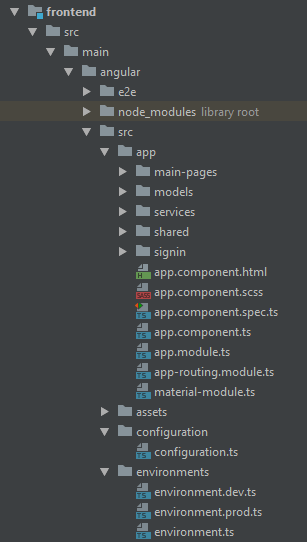
\includegraphics[scale=0.70]{package_structure_frontend.png}
		\caption[Paketstruktur des Frontends]{Paketstruktur des Frontends}
		\label{fig:package_structure_frontend}
	\end{center}
\end{figure}

\subsection{Environment-Konfiguration}
Die Konfiguration der Environments gestaltet sich sehr einfach. Durch das Hinzufügen eines Codesnippets Listing \ref{lst:angular.json} in die \textit{angular.json}-Datei wird beim Starten der Anwendung mit dem Parameter \textit{-{}-configuration=<environment>} die Datei \textit{environment.ts} mit der Datei environment.<environment>.ts ausgetauscht. Z.B. beim Start der Anwendung mit dem Befehl:
\begin{lstlisting}[language=bash]
$	ng serve --configuration=dev
\end{lstlisting}
 
wird anstatt der Datei environment.ts die Datei environment.dev.ts verwendet. In dieser Datei sind die URL´s zum Backend beim Deployment in OpenShift konfiguriert.

\begin{lstlisting}[language=json, caption={angular.json}, label={lst:angular.json}]
	...
	"configurations": {
		"dev": {
			"fileReplacements": [
			{
				"replace": "src/environments/environment.ts",
				"with": "src/environments/environment.dev.ts"
			}
		]
	},
	...
\end{lstlisting}

\subsection{Konfiguration}
In der configuration.ts-Datei sind die einzelnen Seiten und ein HTTP-Header definiert.

\begin{lstlisting}[language=JavaScript, caption={configuration.ts}, label={lst:configuration.ts}]
	export const configuration = {
		...
		PAGES: {
			HOME: '/home',
			ADDPARTNER: '/addpartner',
			PARTNER: '/partner',
			ADDCOMPANY: '/addcompany',
			COMPANY: '/company',
			LOGIN: '/login'
		},
		...
	}
\end{lstlisting}
Auf den Parameter \textit{HOME} im Listing \ref{lst:configuration.ts} kann im TypeScript-Code mittels \textit{configuration.PAGES.HOME} zugegriffen werden.

\subsection{Anwendung}
In der Anwendung können die Geschäftsfälle \textit{Unternehmen hinzufügen}, \textit{Unternehmen löschen}, \textit{Unternehmen anzeigen} und \textit{Partner anzeigen} abgewickelt werden. Die Logik für diese Geschäftsfälle ist im Verzeichnis \textit{main-pages} enthalten.
Je nach derzeitiger URL wird auf die richtige Komponente geroutet. Die Routing-Regeln sind in der Datei \textit{app-routing.module.ts} definiert. Ein Ausschnitt dieser Datei wird in Listing \ref{lst:app-routing.module.ts} gezeigt.

\begin{lstlisting}[language=JavaScript, caption={app-routing.module.ts}, label={lst:app-routing.module.ts}]
	export const routes: Routes = [
		...
		{
			path: 'home',
			component: MainLayoutComponent,
			loadChildren: () => HomePagesModule,
			data: {pageTitle: 'Home'},
			canActivate: [UserAuthenticationGuard]
		},
		...
\end{lstlisting}
Diese Komponente ist unter dem Pfad \glqq /home\grqq{} erreichbar Die Komponente \textit{MainLayoutComponent} wird dadurch inklusive dem Kindmodul \textit{HomePagesModule} gerendert. Der Header und die Navigation sind in der MainLayoutComponent definiert. Diese lädt danach die HomePagesModule hinzu, in der die eigentliche Logik stattfindet. Durch den \textit{UserAuthenticationGuard} wird überprüft, ob der eingeloggte User diese Seite aufrufen darf.

Für die REST-Aufrufe werden Services verwendet. In diesen wird der HttpClient von Angular injiziert. Dadurch können einfach verschiedene REST-Methoden ausgeführt werden.
Listing \ref{lst:partner.service.ts} zeigt einen Ausschnitt der Datei \textit{partner.service.ts}:

\begin{lstlisting}[language=JavaScript, caption={partner.service.ts}, label={lst:partner.service.ts}]
	export class PartnerService {
		...
		private readonly URL = environment.backendOriginSegment + ":" +
			environment.backendOriginPort;
		
		constructor(private http: HttpClient) {}
	
		addOrUpdatePartner(id: number, partner: Partner): Observable<Partner> {
			return this.http.post<Partner>(this.URL + "/company/" + id + "/partner",
				JSON.stringify(partner, partner.constructor.prototype),
					.pipe(
						retry(1)
					);
		}
		...
	}
\end{lstlisting}
Durch die environment-Datei wird die URL aus Host und Port zusammengebaut. Dadurch wird sichergestellt, dass lokal und in OpenShift die richtige URL für das Backend verwendet wird, ohne Code ändern zu müssen.

Beim Aufruf der Methode \textit{addOrUpdatePartner} wird ein POST-Aufruf zur entsprechenden URL mit dem Objekt \textit{Partner} im Body durchgeführt. Die retry-Pipe gibt an, wie oft dieser Aufruf bei einem Fehlversuch wiederholt werden soll. Diese Methode gibt ein Observable zurück, auf das registriert werden kann. 

Der Aufruf dieser Methode sieht, wie in Listing \ref{lst:addPartner} gezeigt, aus.
\begin{lstlisting}[language=JavaScript, caption={addPartner-Methode}, label={lst:addPartner}]
	addPartner(): void {
		this.addOrUpdatePartnerSubscription = 
			this.partnerService.addOrUpdatePartner(this.selectedCompany.id, this.partner)
				.subscribe((partner: Partner) => {
					...
				})
	}
\end{lstlisting}

Die \textit{addOrUpdatePartner}-Methode im PartnerService wird mittels der UnternehmensID und dem veränderten oder neu hinzugefügten Partner aufgerufen. Dadurch, dass diese Methode ein Observable zurückliefert, kann man sich mittels der Methode \textit{subscribe} auf dieses Observable registrieren. Sobald die Response vom Server kommt, wird der Code in der \textit{subscribe}-Methode aufgerufen.

\subsection{Starten der Anwendung}
\textbf{Lokal} kann das Frontend über folgenden Kommandozeilenbefehl gestartet werden:
\begin{lstlisting}[language=bash]
$ ng serve --configuration=dev
\end{lstlisting}

Mittels dem Parameter \textit{-{}-configuration=dev} wird das lokale Environment gestartet. Mittels \textit{ng serve} wird ein von Angular mitgelieferter Webserver hochgefahren. In diesem läuft die Applikation und kann im Browser unter der URL \textit{http://localhost:4200} aufgerufen werden.

Mit folgendem Befehl kann die Applikation in \textbf{OpenShift} deployt werden:
\begin{lstlisting}[language=bash]
$ npx nodeshift --dockerImage=nodeshift/ubi8-s2i-web-app 
	--imageTag=10.x --build.env OUTPUT_DIR=dist/frontend --expose
\end{lstlisting}

Nodeshift ist ein Kommandozeilentool zum Deployment von Node.js-Anwendungen in OpenShift. Dabei wird das Docker Image \textit{nodeshift/ubi8-s2i-web-app} mit dem Image Tag \textit{10.x} verwendet. 
Das Output-Directory wird auf \textit{dist/frontend} gesetzt. Dies ist das Verzeichnis, in dem die Applikation gebaut wird. Mittels \textit{-{}-expose} wird die Route der Applikation in OpenShift freigegeben und ist damit durch einen Browser erreichbar.